% Compile with XeLaTeX, TeXLive 2013 or more recent
\documentclass{beamer}

% Base packages
\usepackage{fontspec}
\defaultfontfeatures{Scale=MatchLowercase, Mapping=tex-text}

\usepackage{amsfonts}
\usepackage{amsmath}
\usepackage{longtable}
\usepackage{csquotes}
\usepackage{standalone}

\usepackage{graphicx}
\graphicspath{{./images/}}

\usepackage{tikz}
\usetikzlibrary{shapes, calc, arrows, decorations, patterns, chains, fit, petri}
\usetikzlibrary{backgrounds, positioning, decorations.pathreplacing}

\newcommand{\inputpicture}[1]{\input{../pictures/#1}}

\usepackage{tabularx}
\usepackage{multirow}

\usepackage{listings}
\lstset{language=C, basicstyle=\ttfamily, breaklines=true, keepspaces=true, keywordstyle=\color{blue}}

% Setup fonts
\newfontfamily\russianfont{CMU Serif}
\setromanfont{CMU Serif}
\setsansfont{CMU Sans Serif}
%\setmonofont{CMU Typewriter Text}

% Be able to insert hyperlinks
\usepackage{hyperref}
\hypersetup{colorlinks=true, linkcolor=black, filecolor=black, citecolor=black, urlcolor=blue , pdfauthor=Evgeny Yulyugin <yulyugin@gmail.com>, pdftitle=Параллельное программирование}
% \usepackage{url}

% Misc optional packages
\usepackage{underscore}
\usepackage{amsthm}

% A new command to mark not done places
\newcommand{\todo}[1][]{{\color{red}TODO\ #1}}

\newcommand{\abbr}{\textit{англ.}\ }

\newif\ifmipt
\newif\ifsbertech
\input{target}

\ifmipt
\subtitle{Курс <<Параллельное программирование>>}
\fi
\ifsbertech
\subtitle{Курс <<Инфраструктура многопроцессорных систем>>}
\fi
\subject{Лекция}
\author[Евгений Юлюгин]{Евгений Юлюгин \texorpdfstring{\\}{Lg} \small{\href{mailto:yulyugin@gmail.com}{yulyugin@gmail.com}}}
\date{\today}
\pgfdeclareimage[height=0.5cm]{mipt-logo}{common/mipt.png}
\logo{\pgfuseimage{mipt-logo}}

\typeout{Copyright 2014 Evgeny Yulyugin}

\usetheme{Berlin}
\setbeamertemplate{navigation symbols}{}%remove navigation symbols


\title{Кэш память в многопроцессорных системах}

\begin{document}

\begin{frame}
\titlepage
\end{frame}

\section*{Обзор}

\begin{frame}{На прошлой лекции}
\begin{itemize}
    \item Цикл работы процессора.
    \item Идеальный конвейер.
    \item Реальный конвейер.
\end{itemize}
\end{frame}

\begin{frame}{На этой лекции}
\tableofcontents
\end{frame}

\section{Назначение}

\begin{frame}{Стена памяти}
\begin{figure}
    \centering
    \includegraphics[width=\textwidth]{memory-wall}
\end{figure}
\end{frame}

\begin{frame}{Ускорение доступов в память}
\begin{itemize}
    \item Быстрое, небольшое хранилище,
    \item Прозрачно для ISA,
    \item Хранит недавно использованные блоки, а также прилегающие к ним данные.
\end{itemize}
\end{frame}

\begin{frame}{Локальность (\abbr locality) данных}
\centering
\resizebox{8cm}{6cm}{
\inputpicture{locality}
}
\end{frame}

\section{Устройство и принципы работы}

\begin{frame}{Кэш (\abbr cache)}
\centering
\inputpicture{cache}
\end{frame}

\begin{frame}{Поиск в кэше}
\begin{figure}[htpb]
    \centering
    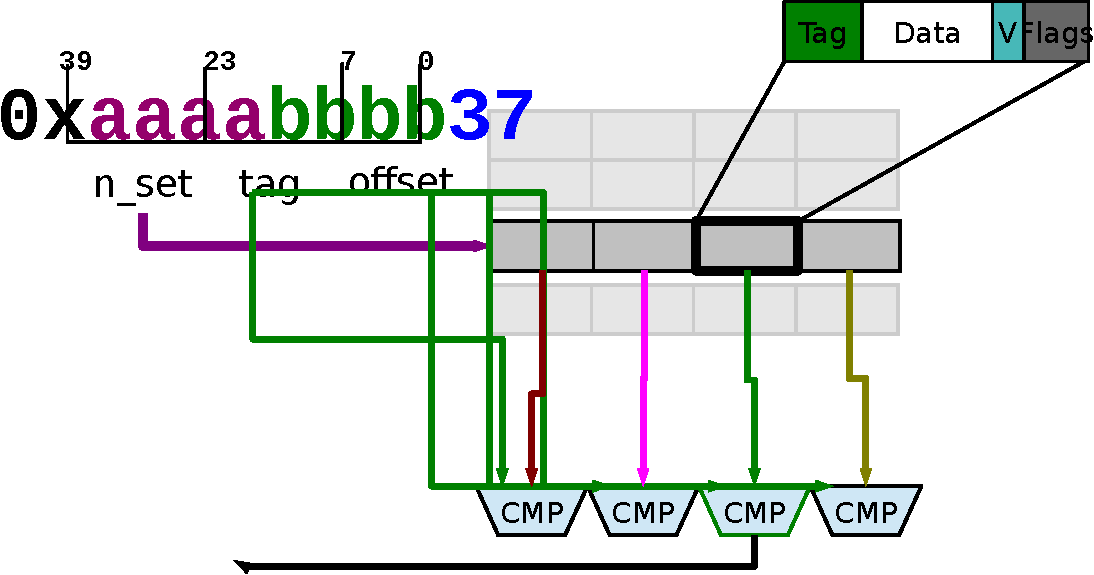
\includegraphics[width=0.65\textwidth]{cache-search}
\end{figure}
\end{frame}

\begin{frame}{Ассоциативность}
\begin{figure}[htpb]
    \centering
    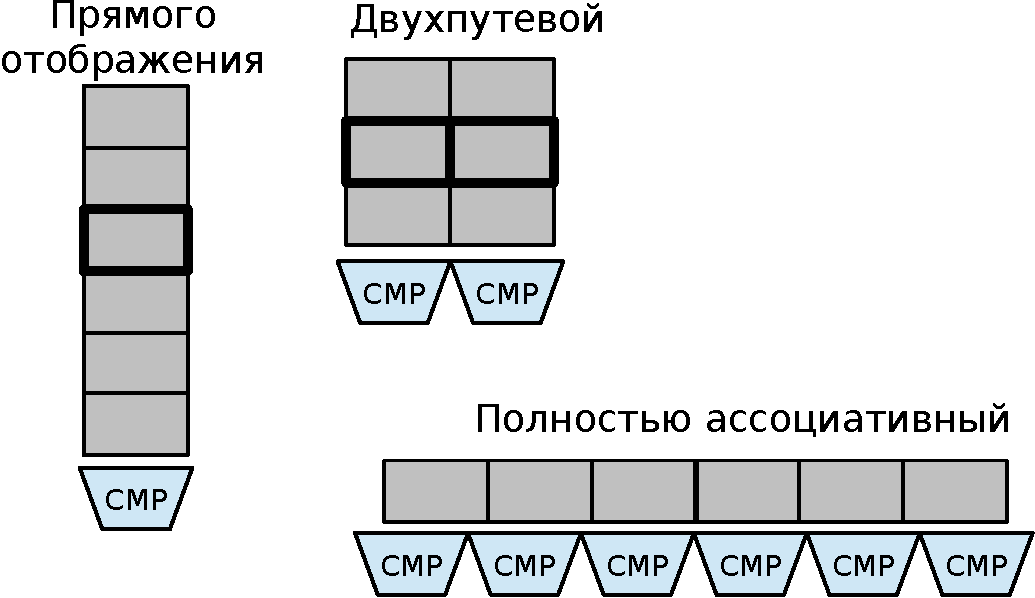
\includegraphics[width=0.65\textwidth]{associativity}
\end{figure}
\end{frame}

\begin{frame}{События при поиске в кэше}
\begin{columns}[t]
    \begin{column}[T]{0.5\textwidth}
    Внешние:
    \begin{itemize}
        \item Чтение --- попадание,
        \item Чтение --- промах,
        \item Запись --- попадание,
        \item Запись --- промах.
    \end{itemize}
    \end{column}
    \begin{column}[T]{0.5\textwidth}
    Внутренние:
    \begin{itemize}
        \item Поиск --- тэг не найден,
        \item Поиск --- флаг V снят,
        \item Добавление --- нет свободной ячейки.
    \end{itemize}
    \end{column}
\end{columns}
\end{frame}

\begin{frame}{Кэши и физические/виртуальные адреса}
\begin{figure}[htpb]
    \centering
    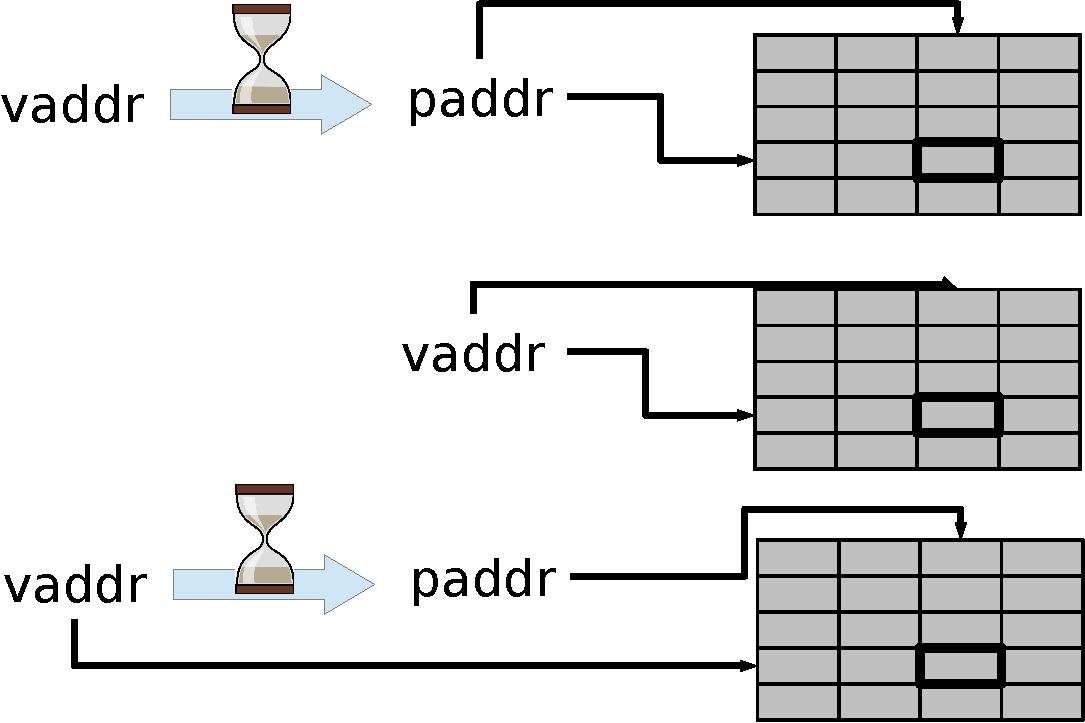
\includegraphics[width=0.65\textwidth]{cache-addressing}
\end{figure}
\end{frame}

\begin{frame}{Кэш инструкций и данных}
\centering
\inputpicture{instr-data-cache}
\end{frame}

\begin{frame}{Многоуровневые кэши}
\begin{itemize}
    \item Один уровень кэша имеет ограничения по емкости/скорости,
    \item Решение --- ирархическая система,
    \item Кэши высоких уровней имеют большую емкости и большее время доступа.
\end{itemize}
\end{frame}

\begin{frame}{Многоуровневые кэши}
\centering
\inputpicture{l1l2}
\end{frame}

\begin{frame}{Политики записи в память}
\begin{itemize}
    \item WT (write through),
    \item WB (write back),
    \item WA (write allocate),
    \item WC (write combined),
    \item UC (uncacheable).
\end{itemize}
\end{frame}

\section{Кэши в многопроцессорных системах}

\begin{frame}{Кэши в многопроцессорных системах}
\begin{itemize}
    \item В качастве кэширующих агентов выступают CPU/другие устройства, имеющие DMA,
    \item Исполняющимся программам необходимо иметь <<консистентный>> вид на память,
    \item Обеспечивается подшлядыванием в чужие кэши/явными передачами
    сообщений и определяется протоколом когерентности системы.
\end{itemize}
\end{frame}

\begin{frame}{Когерентность}
\begin{table}[htpb]
    \begin{center}
    \begin{tabular}{|l|r|r|r|}
    \hline
    \diaghead{0.00001\hskip 0.07\hsize}{Адрес}{CPU} &   CPU0    &   CPU1    &   CPU2    \\
    \hline
    0xaabbccd0 & \textcolor{red}{0x15}   & \textcolor{red}{0x12}   & \#\#\#                  \\
    \hline
    0xaabbcce0 & \textcolor{green}{0x11} & \textcolor{green}{0x11} & \textcolor{green}{0x11} \\
    \hline
    \end{tabular}
    \end{center}
\end{table}
\end{frame}

\begin{frame}{MESI}
\inputpicture{mesi}
\end{frame}

\section*{Конец}
% The final "thank you" frame

\begin{frame}[allowframebreaks]{Литература}
\begin{thebibliography}{99}
    \bibitem{urlich-cpumemory} \textit{Urlich Drepper}. What Every Programmer
    Should Know About Memory.
    \url{http://www.cs.bgu.ac.il/~os142/wiki.files/drepper-2007.pdf}
    \bibitem{henecy-patterson} \textit{John L. Hennessy and David A. Patterson}.
    Computer Architecture -- A Quantitative Approach (5. ed.).
\end{thebibliography}
\end{frame}

\begin{frame}{На следующей лекции}
\begin{itemize}
    \item Графические процессоры.
    \item Сравнительный анализ графического и центрального процессора.
\end{itemize}
\end{frame}

\begin{frame}

{\huge{Спасибо за внимание!}\par}

\vfill

\tiny{\textit{Замечание}: все торговые марки и логотипы, использованные в данном материале, являются собственностью их владельцев. Представленная здесь точка зрения отражает личное мнение автора, не выступающего от лица какой-либо организации.}

\end{frame}

\end{document}
